\documentclass{article}

\usepackage[final]{neurips_2023}
\usepackage[utf8]{inputenc}
\usepackage[T1]{fontenc}
\usepackage{hyperref}
\usepackage{url}
\usepackage{booktabs}
\usepackage{amsfonts}
\usepackage{nicefrac}
\usepackage{microtype}
\usepackage{xcolor}
\usepackage{graphicx}
\usepackage{float}
\graphicspath{{../figures/}{./}}

\title{MLPC 2026 Task 5: The Challenge}

\author{%
  Team Unified Decoders \AND
  Alexandre Escudier Agostinho
  \And
  Jakob Hinterholzer
}

\begin{document}

\maketitle

\section{Baseline Reproduction}

\subsection{Training and Evaluation of the Baseline}

We reproduced the provided baseline using one binary decision tree classifier per sound event class (15 classifiers total), trained on 50{,}000 segments subsampled from the 170{,}508 training segments (960 features per segment). Predictions are generated for overlapping 1-second segments with 0.5\,s hop, and every second segment is discarded so that only predictions starting at full-second timestamps are retained. Using the official evaluation script, we obtain a Segment-based Macro F1 Score of \textbf{0.3170} on the non-hidden test set (0.3072 on the local validation set). Figure~\ref{fig:baseline-bars} shows the per-class F1 scores, and Table~\ref{tab:baseline-perclass} reports per-class precision, recall, and F1 on the non-hidden test set, together with the class frequency in the training set.

\begin{figure}[H]
  \centering
  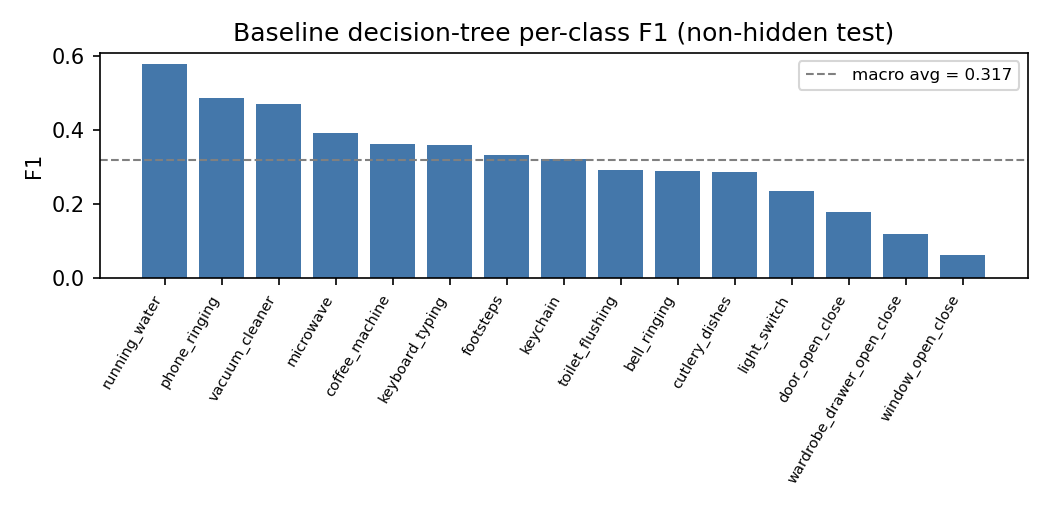
\includegraphics[width=0.95\linewidth]{baseline_perclass_f1.png}
  \caption{Per-class F1 of the baseline decision tree system on the non-hidden test set; the dashed line marks the macro average ($0.317$).}
  \label{fig:baseline-bars}
\end{figure}

\begin{table}[H]
  \caption{Per-class results of the baseline on the non-hidden test set, sorted by F1.}
  \label{tab:baseline-perclass}
  \centering
  \small
  \begin{tabular}{lrrrr}
    \toprule
    Class & Precision & Recall & F1 & Train Freq.\ \\
    \midrule
    running\_water              & 0.655 & 0.517 & \textbf{0.578} & 13.6\% \\
    phone\_ringing              & 0.534 & 0.444 & 0.485 & 7.6\% \\
    vacuum\_cleaner             & 0.485 & 0.455 & 0.470 & 6.7\% \\
    microwave                   & 0.408 & 0.373 & 0.390 & 7.5\% \\
    coffee\_machine             & 0.504 & 0.283 & 0.362 & 3.8\% \\
    keyboard\_typing            & 0.372 & 0.347 & 0.359 & 10.4\% \\
    footsteps                   & 0.385 & 0.293 & 0.333 & 14.4\% \\
    keychain                    & 0.365 & 0.287 & 0.321 & 5.8\% \\
    toilet\_flushing            & 0.288 & 0.292 & 0.290 & 3.4\% \\
    bell\_ringing               & 0.426 & 0.218 & 0.288 & 1.5\% \\
    cutlery\_dishes             & 0.294 & 0.281 & 0.287 & 7.9\% \\
    light\_switch               & 0.240 & 0.228 & 0.234 & 1.6\% \\
    door\_open\_close           & 0.200 & 0.159 & 0.177 & 5.5\% \\
    wardrobe\_drawer\_open\_close & 0.134 & 0.109 & 0.120 & 3.0\% \\
    window\_open\_close         & 0.057 & 0.066 & 0.061 & 2.1\% \\
    \midrule
    \textbf{Macro Average}      & --    & --    & \textbf{0.317} & -- \\
    \bottomrule
  \end{tabular}
\end{table}

\subsection{Performance Differences Between Classes}

The per-class results form three tiers driven more by acoustic nature and duration than by raw class frequency. \textbf{Sustained, distinctive sounds dominate}: the top performers (running\_water 0.58, phone\_ringing 0.49, vacuum\_cleaner 0.47, microwave 0.39) last several seconds and fill the 1-second window with clean positives, and their spectral signatures (broadband noise, periodic ringing) are well captured by MFCC/mel features. \textbf{Frequency alone does not predict performance}: footsteps is the most frequent class (14.4\%) yet ranks only 7th (0.33), while coffee\_machine is rarer (3.8\%) but ranks 5th (0.36); footsteps, keychain (0.32) and cutlery\_dishes (0.29) are short impact sounds that resemble each other and other impacts, hard to separate from 1-second statistics. \textbf{Short transients are systematically hardest}: the four worst classes are the briefest events --- window (0.06), wardrobe (0.12), door (0.18), light\_switch (0.23) --- often well below 1\,s, so the aggregating window dilutes them with background and inherits label noise from partially-covered segments. \textbf{Precision exceeds recall almost everywhere} (avg.\ 0.36 vs.\ 0.28): on imbalanced data the trees default to the negative class, giving a conservative detector that is usually right when it fires but misses many events (e.g.\ bell\_ringing 0.43/0.22).

\subsection{Strengths and Limitations of the Baseline}

\textbf{Strengths.} The baseline is simple, interpretable, and consistent between validation and test (0.307 vs.\ 0.317), so the training subsample is representative and the trees do not overfit. Independent binary classifiers naturally fit the polyphonic multi-label setting, and the rich feature representation (MFCCs, mel spectrogram, spectral and energy statistics with mean/std/min/max aggregations) captures sustained sounds robustly while tree models tolerate the heterogeneous feature scales without normalization.

\textbf{Limitations.} Four design choices explain most errors: (1)~a single tree cannot represent smooth boundaries in 960-dimensional space, motivating ensembles or feature-interaction models; (2)~independent per-class classifiers ignore co-occurrence (footsteps+door, cutlery+water) that could disambiguate similar impacts; (3)~the fixed 1-second window is mismatched to sub-second transients, mixing the event with silence and lowering its signal-to-noise ratio --- the main reason transient events sit at the bottom of Table~\ref{tab:baseline-perclass}; and (4)~segments are classified independently, so predictions flicker within an event, and the discarded half-second segments waste information.

\section{Simple Classifier}

\subsection{The Best Previous-Phase Classifier: CatBoost}

In the previous project phase we compared a one-vs-rest linear SVM against \textbf{CatBoost} gradient-boosted decision trees, training one binary model per class. CatBoost was the clear winner, reaching a macro-F1 of \textbf{0.535} on the Task-4 split versus \textbf{0.480} for the tuned SVM. The key idea is to grow an additive ensemble of shallow trees, each fit to the gradient of the previous ensemble's error, so the model expresses smooth nonlinear feature interactions that a single decision tree (as used by the baseline) cannot represent. We chose CatBoost for three reasons that fit the data directly: tree splits are invariant to feature scale, so the heterogeneous feature set is consumed without normalization; boosting captures the nonlinear interactions needed to separate acoustically similar impact sounds; and \texttt{auto\_class\_weights="Balanced"} counters the strong class imbalance without resampling. The most important hyperparameters are the tree \emph{depth} (interaction order), the \emph{learning\_rate} (per-tree step size), the number of \emph{iterations}, and the \emph{l2\_leaf\_reg} leaf-regularization.

\subsection{From Baseline Trees to CatBoost in the SED Pipeline}

We replaced the baseline's 15 independent binary decision trees with 15 one-vs-rest CatBoost classifiers in the same segment-level SED pipeline. The decisive challenge-specific enhancement is \textbf{temporal context}: each 1-second segment is augmented with the features of its $\pm2$ neighbouring segments, concatenated per recording and edge-padded at the boundaries. Because neighbouring evidence helps localise and disambiguate events in the SED setting, this single change raised macro-F1 from the Task-4-style \textbf{0.535} to \textbf{0.584} on the challenge non-hidden test set.

\textbf{Hyperparameter study.} We swept the three most influential knobs one at a time around the defaults on the base feature set (Table~\ref{tab:cb-hp}). Tree \emph{depth} peaks at $6$ (shallower underfits, deeper does not help); the \emph{learning\_rate} is flat up to $0.1$ but $0.2$ overshoots and collapses to $0.521$; and a slightly stronger \emph{l2\_leaf\_reg} of $6$ marginally beats the default. Otherwise the curves are flat, all within $\approx0.006$ macro-F1, confirming that CatBoost is robust to these settings. The final configuration is 15 one-vs-rest CatBoost classifiers with $1500$ iterations, \texttt{learning\_rate}~$=0.05$, \texttt{depth}~$=6$, \texttt{l2\_leaf\_reg}~$=3$, \texttt{auto\_class\_weights="Balanced"}, per-class probability thresholds tuned on the validation set, and the $\pm2$ temporal window.

\begin{table}[H]
  \caption{Validation macro-F1 of the CatBoost coordinate sweep (one knob varied at a time around the defaults). Selected values in \textbf{bold}.}
  \label{tab:cb-hp}
  \centering
  \small
  \begin{tabular}{lllll}
    \toprule
    \texttt{depth}          & 4: 0.531    & \textbf{6: 0.537}    & 8: 0.536  & 10: 0.535 \\
    \texttt{learning\_rate} & 0.02: 0.534 & \textbf{0.05: 0.537} & 0.1: 0.537 & 0.2: 0.521 \\
    \texttt{l2\_leaf\_reg}  & 1: 0.534    & 3: 0.537             & \textbf{6: 0.540} & 10: 0.538 \\
    \bottomrule
  \end{tabular}
\end{table}

\subsection{Comparison Against the Baseline}

The final CatBoost system raises overall Macro-F1 from the baseline's \textbf{0.317} to \textbf{0.584} on the challenge non-hidden test set, a $+0.267$ absolute gain ($\approx1.84\times$). Table~\ref{tab:cb-compare} reports the per-class breakdown, sorted by improvement.

\begin{table}[H]
  \caption{Per-class F1 on the challenge non-hidden test set, baseline decision trees vs.\ final CatBoost, sorted by improvement. CatBoost precision/recall also shown. Only \emph{light\_switch} regresses.}
  \label{tab:cb-compare}
  \centering
  \small
  \begin{tabular}{lrrrrr}
    \toprule
    Class & Base F1 & CB P & CB R & CB F1 & $\Delta$F1 \\
    \midrule
    keyboard\_typing            & 0.359 & 0.823 & 0.822 & \textbf{0.822} & $+0.463$ \\
    cutlery\_dishes             & 0.287 & 0.689 & 0.684 & 0.686 & $+0.399$ \\
    toilet\_flushing            & 0.290 & 0.789 & 0.588 & 0.674 & $+0.384$ \\
    keychain                    & 0.321 & 0.750 & 0.629 & 0.684 & $+0.363$ \\
    footsteps                   & 0.333 & 0.632 & 0.664 & 0.648 & $+0.315$ \\
    window\_open\_close         & 0.061 & 0.354 & 0.378 & 0.365 & $+0.304$ \\
    vacuum\_cleaner             & 0.470 & 0.818 & 0.733 & 0.773 & $+0.303$ \\
    door\_open\_close           & 0.177 & 0.469 & 0.472 & 0.470 & $+0.293$ \\
    coffee\_machine             & 0.362 & 0.665 & 0.620 & 0.642 & $+0.280$ \\
    microwave                   & 0.390 & 0.699 & 0.593 & 0.642 & $+0.252$ \\
    running\_water              & 0.578 & 0.823 & 0.766 & 0.793 & $+0.215$ \\
    wardrobe\_drawer\_open\_close & 0.120 & 0.280 & 0.356 & 0.313 & $+0.193$ \\
    phone\_ringing              & 0.485 & 0.567 & 0.714 & 0.632 & $+0.147$ \\
    bell\_ringing               & 0.288 & 0.360 & 0.496 & 0.417 & $+0.129$ \\
    light\_switch               & 0.234 & 0.163 & 0.262 & 0.201 & $-0.033$ \\
    \midrule
    \textbf{Macro Average}      & \textbf{0.317} & 0.592 & 0.585 & \textbf{0.584} & $+0.267$ \\
    \bottomrule
  \end{tabular}
\end{table}

\textbf{The largest gains land exactly where the baseline was weakest.} The biggest improvements are on short impulsive, transient, and kitchen sounds --- \emph{keyboard\_typing} ($+0.463$), \emph{cutlery\_dishes} ($+0.399$), \emph{toilet\_flushing} ($+0.384$), \emph{keychain} ($+0.363$), \emph{footsteps} ($+0.315$), and the open/close events --- precisely the classes Section~1 identified as the hardest tier. We attribute this to two complementary effects: gradient-boosted ensembles capture nonlinear feature interactions that a single tree cannot, and the $\pm2$ temporal context supplies neighbouring evidence that helps localise brief events whose signal is otherwise diluted within a 1-second window.

\textbf{Precision and recall are now balanced.} Whereas the baseline was precision-skewed and conservatively under-predicting (Section~1), CatBoost reaches macro precision $0.592$ and recall $0.585$ --- the balanced class weights and per-class tuned thresholds corrected the baseline's tendency to default to the negative class.

\textbf{One class regresses.} \emph{light\_switch} is the sole regression ($0.234\!\rightarrow\!0.201$) and remains the hardest class. It is the rarest, briefest, sub-second transient with no characteristic spectrum, so temporal context offers no leverage when the event is itself acoustically featureless; the balanced weighting then inflates false positives, dragging precision to $0.163$.

\subsection{Qualitative Error Analysis}

We inspect the detector on two test recordings from unseen collectors, overlaying predicted vs.\ expected per-class timelines (green = correct, red = false alarm, blue = missed, grey = true negative).

\textbf{File 002675} (Figure~\ref{fig:cs1}) is a busy scene. The central \emph{footsteps} block is detected almost perfectly, but \emph{footsteps} over-fires in earlier unannotated segments --- high recall, low precision for this impulsive broadband class. \emph{running\_water} shows the opposite failure, latching onto the onset and then losing the sustained stretch, while \emph{cutlery\_dishes} is missed entirely. \textbf{File 000118} (Figure~\ref{fig:cs2}, left) is dominated by a vacuum cleaner that is largely missed outside its loudest portion, despite its strong overall F1 ($0.773$): the model keys on intensity rather than the spectral signature, so the quieter onset and tail are lost. \emph{running\_water} at the start is detected cleanly, and \emph{footsteps} again mixes a correct block with scattered false alarms. The cross-class confusion matrix (Figure~\ref{fig:cs2}, right) shows the residual errors are perceptually plausible rather than random --- bell$\leftrightarrow$phone (both tonal ringing), door$\leftrightarrow$window (near-identical open/close events), and cutlery$\leftrightarrow$water/keychain (clattering kitchen sounds that co-occur) --- and the near-empty \emph{light\_switch} row confirms it almost never fires confidently, consistent with its bottom-ranked F1.

\section{Post-Processing and Temporal Refinement}

Because the 15 classifiers predict each second independently, a class's activity sequence can flicker between active and inactive within a single event. We investigate \textbf{temporal median filtering}: each per-second binary prediction is replaced by the median of a sliding window of $w$ consecutive predictions of the same class within the same recording, applied before consecutive active seconds are merged into onset/offset intervals. This removes isolated single-second activations and fills single-second gaps while preserving longer event regions.

\textbf{Effect of the window size.} Figure~\ref{fig:postproc} reports segment macro-F1 on the test split as the window grows. The effect is small and quickly negative: a minimal window of $w=3$ yields a negligible gain ($0.5842\!\rightarrow\!0.5848$, $+0.0006$), while every larger window degrades performance monotonically --- $w=5$: $0.573$ ($-0.011$), $w=7$: $0.557$ ($-0.027$), $w=9$: $0.543$ ($-0.041$).

\begin{figure}[H]
  \centering
  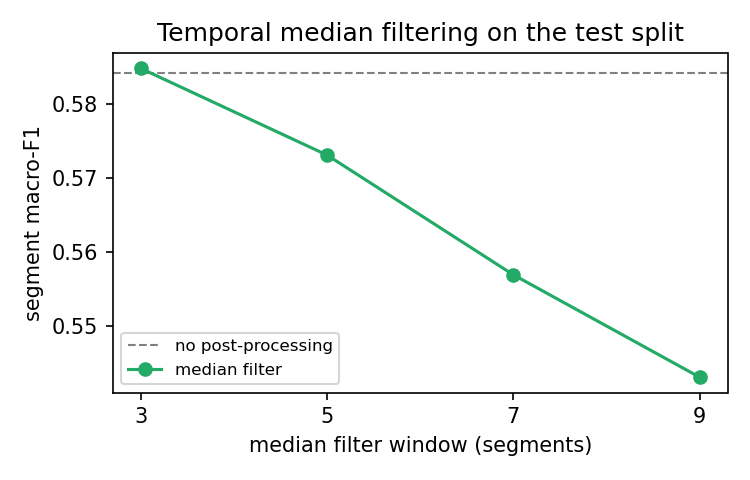
\includegraphics[width=0.5\linewidth]{postproc_median.png}
  \caption{Segment macro-F1 on the test split vs.\ median-filter window size; the dashed line is the unfiltered system ($0.5842$). Only the minimal $w=3$ window helps, marginally.}
  \label{fig:postproc}
\end{figure}

\textbf{Interpretation.} The limited headroom follows from earlier design choices: the $\pm2$ temporal-context features and per-class tuned thresholds already yield temporally coherent predictions, so little isolated flicker remains for a median filter to clean. Conversely, wider windows erase genuinely short events faster than they remove noise --- the sub-second transients (\emph{light\_switch}, \emph{door}, \emph{window}), often only one or two seconds long, are smoothed away entirely, lowering their recall and dragging down the equally-weighted macro average. We therefore retain only the minimal $w=3$ filter in the final system: temporal refinement offers little benefit once temporal context is already encoded in the features.
\section{Reflection and Real-World Considerations}

\textbf{Technical limitations and future work.} Three error sources dominate the final system (macro-F1 $0.584$, per-class $0.822$ for \emph{keyboard\_typing} down to $0.201$ for \emph{light\_switch}). (1)~\emph{Temporal-resolution mismatch.} The fixed 1-second aggregation window is far longer than the sub-second \emph{open/close} transients (\emph{light\_switch} $0.201$, \emph{wardrobe} $0.313$, \emph{window} $0.365$), so a brief event is diluted by the surrounding silence it is summarized with. A model operating at finer resolution --- raw log-mel frames in a CRNN with explicit event-boundary modelling rather than 1\,s summary statistics --- would localize these onsets instead of averaging them away. (2)~\emph{Lost within-segment shape.} The mean/std features discard the temporal evolution inside each second; learned spectrogram features would retain the attack-decay structure that separates an impulsive \emph{door} click from sustained noise. (3)~\emph{Independent per-class detectors.} Training 15 one-vs-rest models ignores the confusion and co-occurrence structure that drives the systematic, perceptually plausible errors --- \emph{bell}$\leftrightarrow$\emph{phone} (both tonal), \emph{door}$\leftrightarrow$\emph{window}, \emph{cutlery}$\leftrightarrow$\emph{water}/\emph{keychain}. A joint multi-label model, or a confusion-aware second stage exploiting which classes co-occur (\emph{footsteps}+\emph{door}, \emph{cutlery}+\emph{water}), could disambiguate same-family sounds. Class imbalance compounds this: rare events (\emph{light\_switch}, \emph{bell\_ringing}) yield noisy, low-precision detectors despite class weighting, which targeted data collection, augmentation, or focal-style losses would directly address. Residual prediction flicker is handled by the temporal smoothing studied in Section~3.

\textbf{Real-world deployment.} As a smart-home component the system is usable but not yet production-grade. A macro-F1 of $0.584$ implies frequent false alarms and misses, concentrated precisely on the brief, convenience-relevant \emph{open/close} events the model is weakest at, so it cannot reliably drive autonomous automations. Robustness is unproven: it was trained and evaluated on this dataset's domestic recordings, whereas real homes present unseen devices, room acoustics, microphone distances, and background sources (TV, conversation) that are under-represented here. Latency is structural --- the $\pm2$-neighbour context requires future segments, so the system lags $\approx 2$\,s behind real time, fine for logging but marginal for responsive control. Its clear strength is efficiency: 15 gradient-boosted trees over cheap MFCC/mel/spectral features run comfortably on an edge hub or on-device, unlike deep alternatives. Reliability, however, is uneven --- per-class quality varies roughly fourfold, so users would find detection dependable for \emph{vacuum\_cleaner}, \emph{keyboard\_typing}, and \emph{running\_water} but erratic for switches and drawers, and always-on home audio raises genuine privacy concerns. In its current state the system is a credible non-critical assistive logger --- low compute, solid on sustained sounds --- but not yet reliable enough for safety-relevant or autonomous action.

\section*{Disclosure of LLM and AI Tool Use}

Claude (Anthropic) and ChatGPT were used to assist with Python implementation of the data processing and classification pipelines, LaTeX formatting, and improving writing clarity. All generated code was tested on our dataset and modified where necessary. All reported results were verified by running the experiments and inspecting the outputs. Content was critically reviewed for technical accuracy before inclusion.

\appendix
\section{Qualitative Error-Analysis Figures}

\begin{figure}[H]
  \centering
  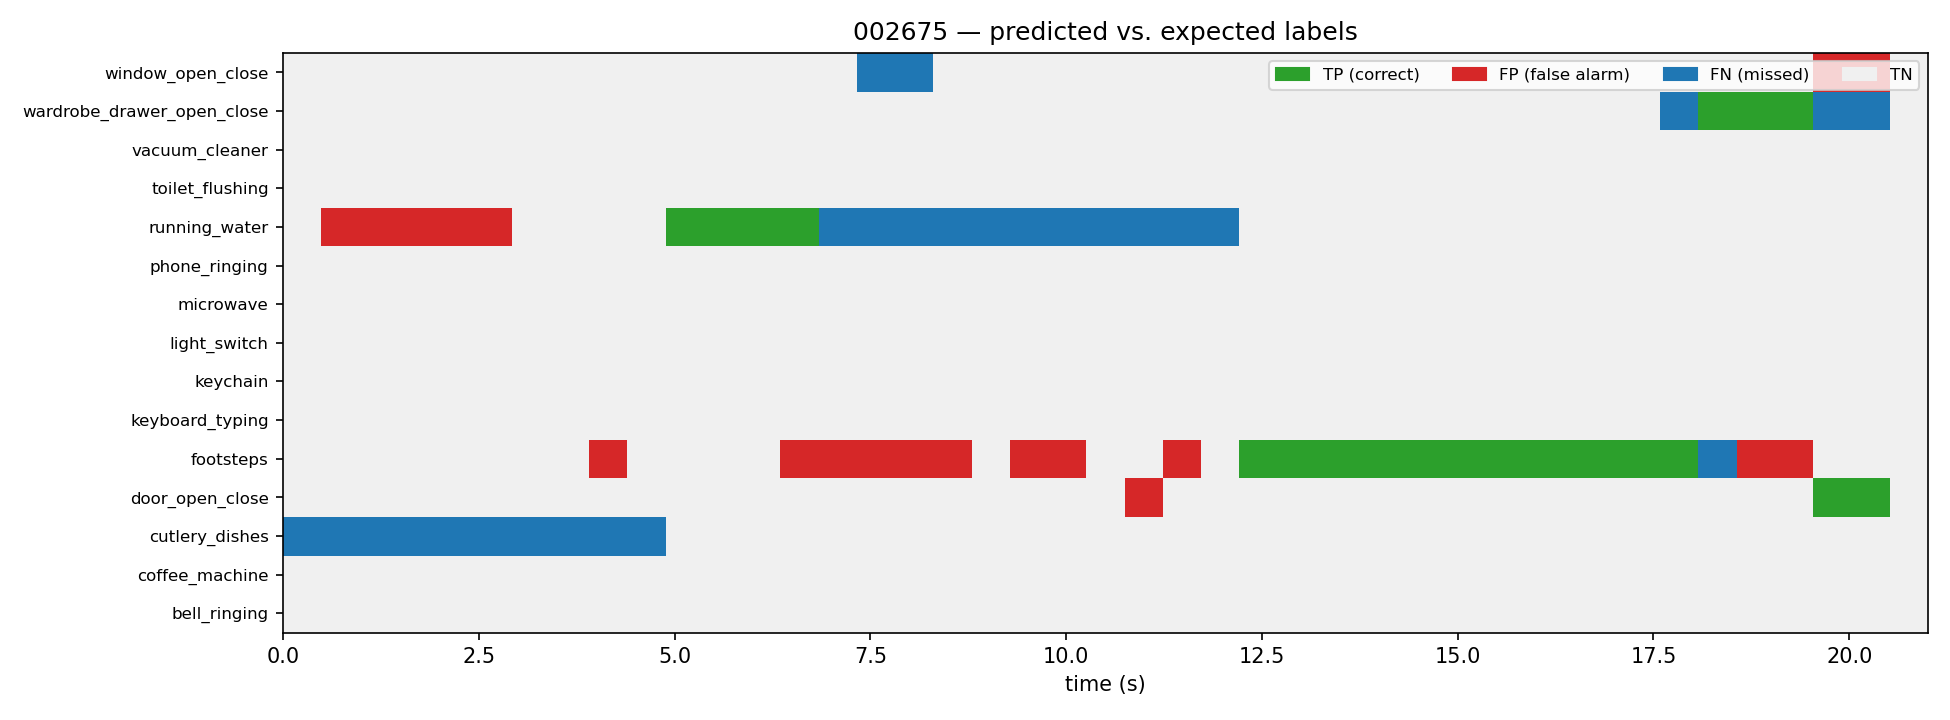
\includegraphics[width=0.7\linewidth]{case_study_002675.png}
  \caption{File 002675 -- predicted vs.\ expected labels per class over time (green = correct, red = false alarm, blue = missed, grey = true negative).}
  \label{fig:cs1}
\end{figure}

\begin{figure}[H]
  \centering
  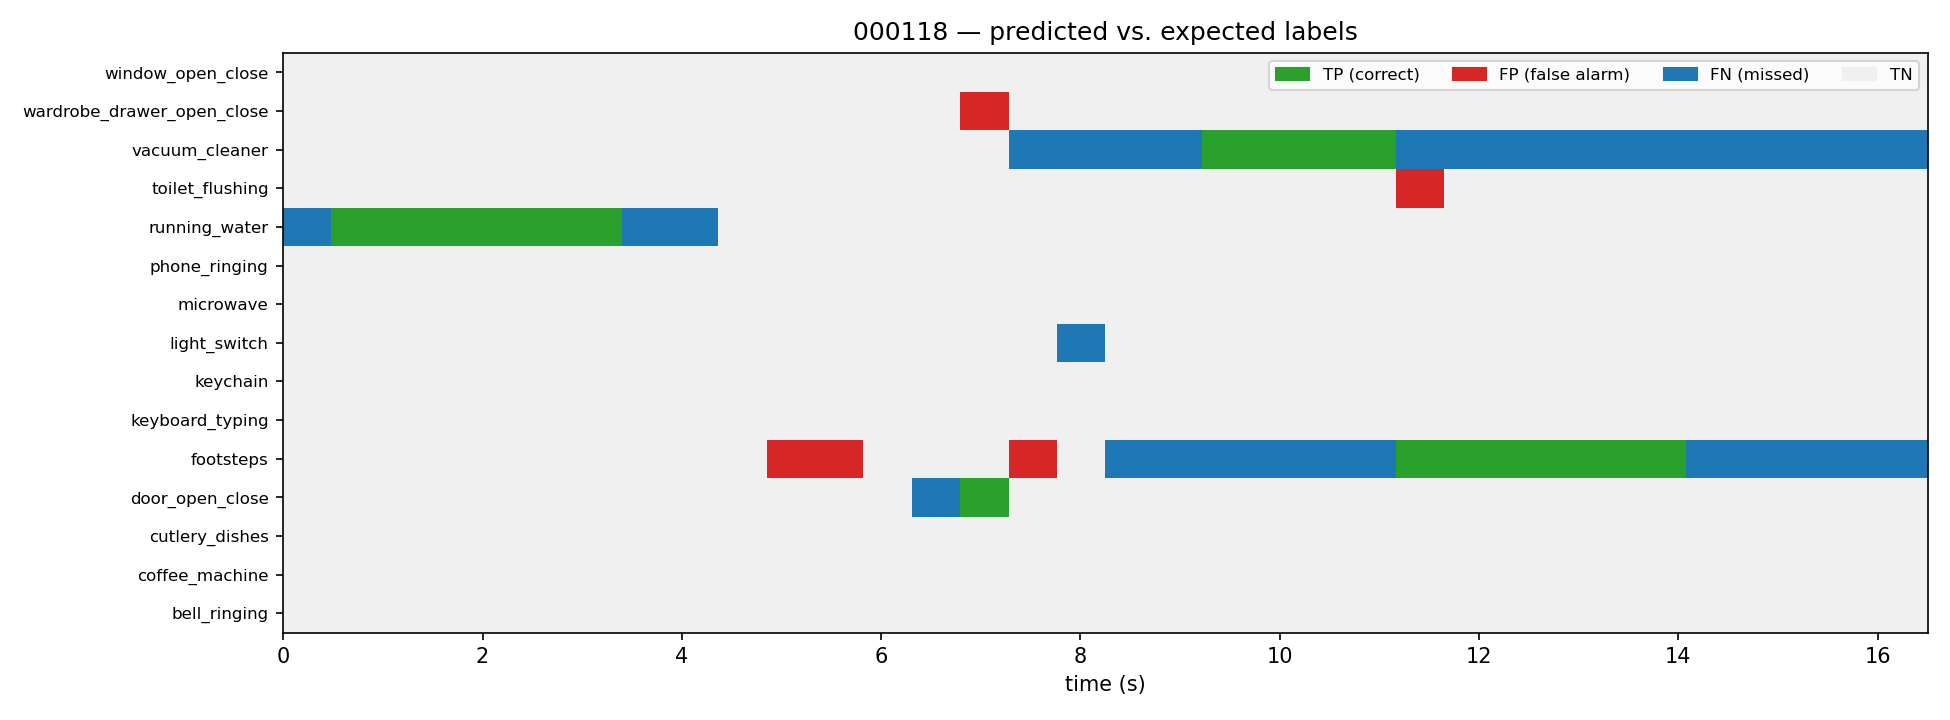
\includegraphics[width=0.6\linewidth]{case_study_000118.png}\hfill
  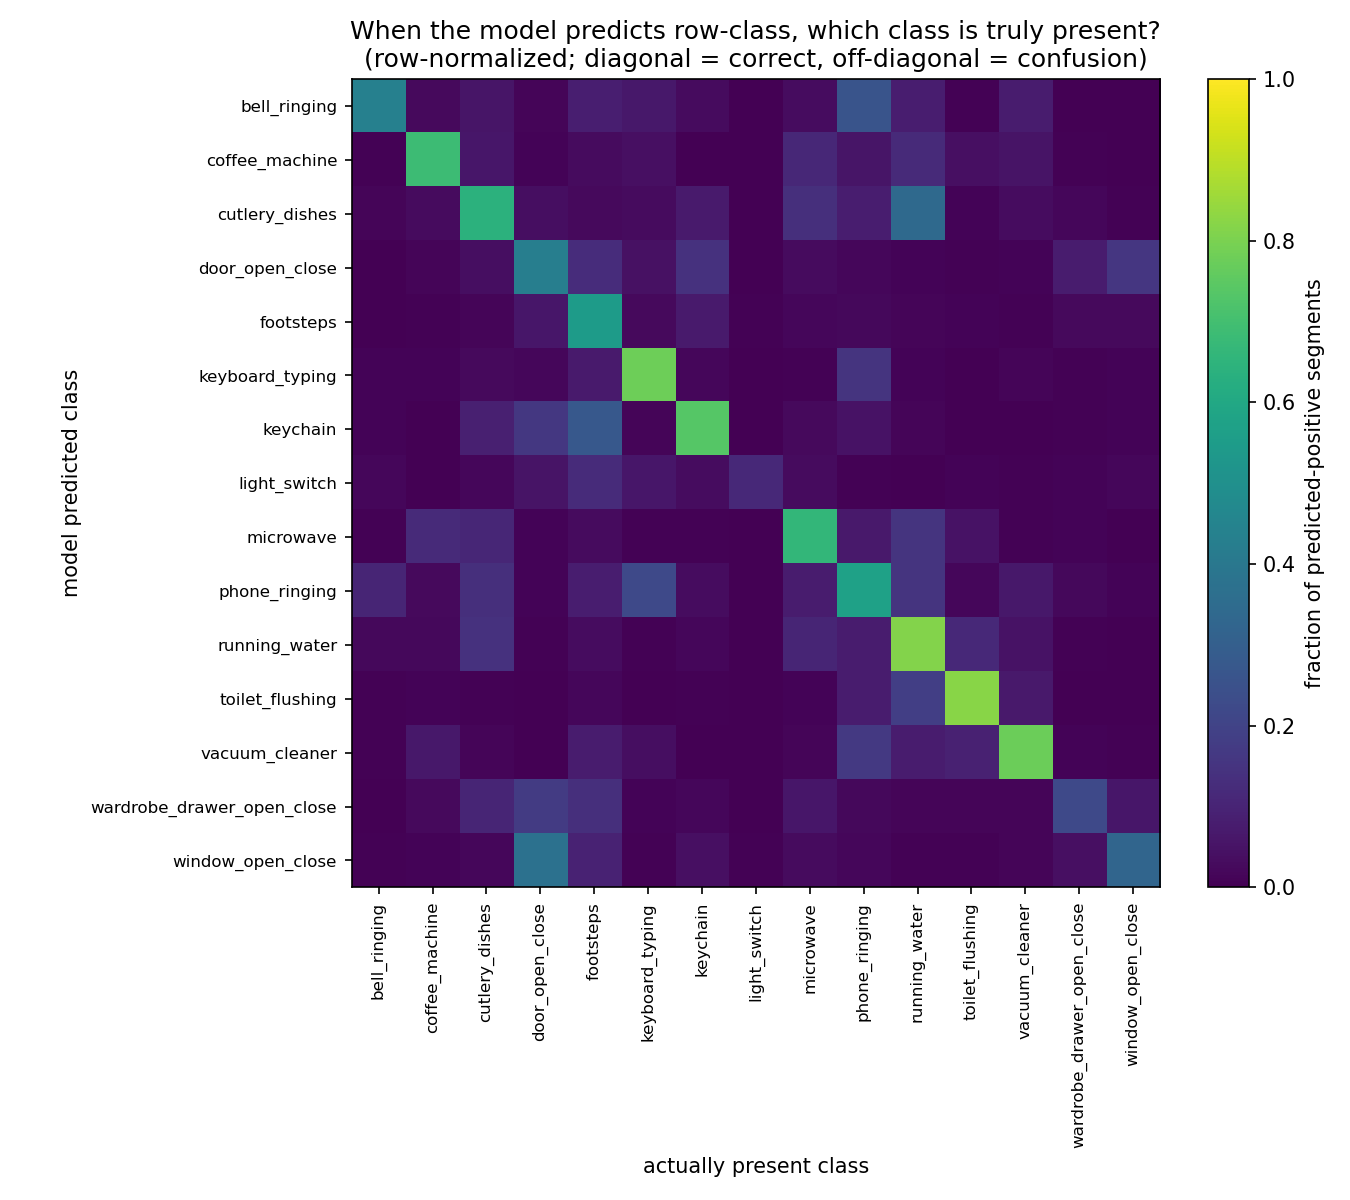
\includegraphics[width=0.38\linewidth]{class_confusion.png}
  \caption{Left: file 000118 -- predicted vs.\ expected labels (same legend as Figure~\ref{fig:cs1}); the vacuum cleaner is mostly missed outside its loudest portion. Right: cross-class confusion; off-diagonal mass marks systematic same-family confusions.}
  \label{fig:cs2}
\end{figure}

\end{document}